\documentclass[11pt]{article}
  \renewcommand{\baselinestretch}{1.05}
  \usepackage{amsmath,amsthm,verbatim,amssymb,amsfonts,amscd,graphicx}
  \usepackage{graphics}
  \usepackage{url}
  \usepackage[utf8]{inputenc}
  \graphicspath{{images/}}
  \topmargin0.0cm
  \headheight0.0cm
  \headsep0.0cm
  \oddsidemargin0.0cm
  \textheight23.0cm
  \textwidth16.5cm
  \footskip1.0cm
  \theoremstyle{plain}
  \newtheorem{theorem}{Theorem}
  \newtheorem{corollary}{Corollary}
  \newtheorem{lemma}{Lemma}
  \newtheorem{proposition}{Proposition}
  \newtheorem*{surfacecor}{Corollary 1}
  \newtheorem{conjecture}{Conjecture}
  \newtheorem{question}{Question}
  \theoremstyle{definition}
  \newtheorem{definition}{Definition}
  \renewcommand{\figurename}{Kuva}

   \begin{document}

  \title{Konvoluutioneuroverkot}
  \author{Teemu Sarapisto}
  \maketitle

  \section{Alkuhommat}

  %Neuroverkot saivat alkunsa jo 40-luvulla, mutta vasta 2006 tarvittavat palaset niiden läpimurtoon saatiin kasaan (katso millaisella kielellä papereita yleensä aloitetaan).

  %Tietokoneiden suorituskyvyn kasvamisen, suurien määrien luokiteltua dataa löytymisen ja sopivien algoritmien kuten backpropagationin  (suomenna) yleistymisen myötä neuroverkot alkoivat noin 2006 alkaen ratkaista ongelmia joihin ei muilla lähestymistavoilla oltu aikaisemmin pystytty. suurta suosiota, oltuaan jo aikaisemmin sekä 40-60 luvuilla, että 80-95 vuosina jo vahvasti pinnalla.

  %Neuroverkot ovat jo pari kertaa olleet pinnalla, mutta niiden todelliseen läpilyömiseen tarvitut osaset löytyivät vasta 2006, kun suuret määrät luokiteltua dataa tuli helposti saataville, ja näytönohjainten tietokoneiden suorituskyvyn kasvettua mm. näytonohjainten hyödyntämisen kautta tarpeeksi suurelle tasolle jotta neuroverkkojen tehokas hyödyntäminen tuli mahdolliseksi. Myös back-propagation.

  Neuroverkot yleistyneet viimeaikoina labeloidun datan määrän kasvettua, tietokoneiden suorituskyvyn kasvettua esimerkiksi näytönohjainten tehokkaan hyödyntämisen kautta jne. Neuroverkkojen lisäkerroksien hyöty löydetty (deep learning). Neuroverkot ottivat vaikutteita biologisista neuroverkoista. neuroverkot erittäin hyviä klassifioimaan kuvia \cite{Goodfellow-et-al-2016}. TODO: paljon yleislätinää neuroverkoista.

  Syväoppiminen blabla erillään?


  \section{Neuroverkkojen rakenne}
  \subsection{Keinotekoinen neuroni}


    Biologisista vaikuttimistaan huolimatta keinotekoiset neuronit ovat käytännössä Kaavan \ref{eq:neuroni} muotoisia matemaattisia funktioita.

    \begin{equation}
      \label{eq:neuroni}
      \Sigma w_i x_i \mapsto f(\Sigma w_i x_i - b)
    \end{equation}

    Yleisessä muodossaan neuroni ottaa vastaan yhden tai useampia syötteitä $x_1$, $x_2$, ..., $x_n$, joista kullekin on asetettu jokin painoarvo $w_i$. Syötteiden ja painotuksien tulojen summa $\Sigma x_i w_i$ annetaan parametrina aktivaatiofunktiolle $f$ ja siitä saatu arvo toimii neuronin lopullisena ulostuloarvona. Joissakin tapauksissa summaparametristä vähennetään ennen funktiolle syöttöä myös taipumusarvo (bias) $b$.

    %You can think of the bias as a measure of how easy it is to get the perceptron to output a 1. Or to put it in more biological terms, the bias is a measure of how easy it is to get the perceptron to fire

    50-luvulla kehitettiin ensimmäinen tällainen neuroni (viittaa niihin perseptronijäbät). Sen syötteet ja ulostuloarvot ovat binäärisiä. Aktivaatiofunktiona toimii vain tarkastus ylittääkö $\Sigma x_i w_i - b$ arvon 0, ja jos, neuronin ulostuloarvo on 1, muuten 0.
    <tähän kaavana threshhold suurempikuin-pienempikuin hommat?>

    Nykyään hyvin yleisesti käytetään sigmoidinen neuroni joka saa nimensä sen aktivaatiofunktiona toimivasta sigmoidisesta funktiosta. Sen syötteet ja paluuarvot ovat reaalilukuja 0 ja 1 väliltä

  %kappaleessa 3 rojanista hyvää juttua \cite{Rojas96}

  %http://neuralnetworksanddeeplearning.com/chap1.html keksi parempi lähde
  % oliko varmasti 50-luvulla?

  \subsection{Verkko neuroneja}

  Yhdessä yksi suuri funktio, joka pystyy mallintamaan mitä tahansa muita funktioita karkeasti tjsp?

  \begin{figure}[h]
  \centering
  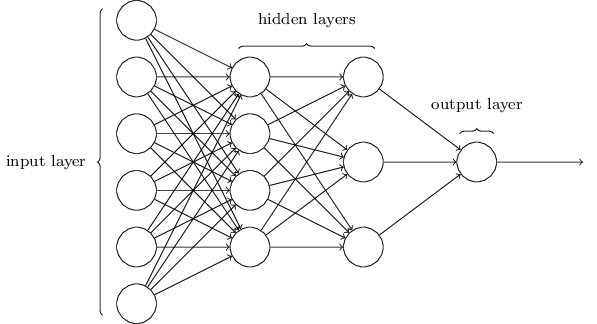
\includegraphics[scale=0.5]{basic-neuralnet}
  \caption{http://neuralnetworksanddeeplearning.com/chap1.html}
  \end{figure}

  Yksinkertaisimman verkkorakenteen omaavat eteenpäinsyöttävät neuroverkot muodostetaan tasoittain, jossa jokaisen verkon tason neuronit saavat syötteenään niitä edeltävän tason neuroneiden ulostuloarvot. Poikkeuksena ensimmäinen taso (kuvassa vasemmanpuoleisimpana), joihin verkon syöte koodataan. Esimerkiksi haluttaessa syöttää 64x64 kuva neuroverkolle, voidaan syötekerroksena käyttää 64x64 neuronin kerrosta, johon kuvan pikselien väriarvot koodataan.


  \section{Neuroverkkojen oppiminen / opettaminen}
  - backpropagation, gradient descent, cost function

  - overfitting

  - (regularization, dropout)

  - weight initialization

  \section{Konvoluutioneuroverkot}
   (For example, the convolutional networks used for object recognition from photos are a specialized kind of feedforward network)
  - Olemassa esim RNN, CNN

  - CNN toimii hyvin kuvien tunnistamiseen. Millaisia CNN:t ovat tarkemmin
  \section{Kuvien tunnistus (konvoluutioneuroverkoilla)}
  - local receptive fields, shared weights/biases, pooling

  \renewcommand{\refname}{Lähteet}
  \bibliographystyle{ieeetr}
  \bibliography{test}

  \end{document}